% Chapter Template

\chapter{INTRODUCCION} % Main chapter title

\label{C1} % Change X to a consecutive number; for referencing this chapter elsewhere, use \ref{ChapterX}

\lhead{Capítulo 1. \emph{INTRODUCCION}} % Change X to a consecutive number; this is for the header on each page - perhaps a shortened title

This brief text is JTLYK that IMHO this Tesis has FMTYEWTK about BMGs. AFAIK their creators: FA, AKA ``El hombre hombre'' and AM, AKA ``El ruludo musical'', recommend you to start reading ASAP. Special THX to EMB and CC.

%----------------------------------------------------------------------------------------
%	SECTION 1
%----------------------------------------------------------------------------------------

\section{Materiales y Vidrios Metálicos.}
\label{S1_1}

Los estados de agregación clásicos de la materia son tres: sólido, líquido y gaseoso. Los sólidos pueden ser clasificados en metales, cerámicos o polímeros. Esta clasificación se basa en la composicion química y la estructura atómica \cite{callister95}. Sin embargo, existe otra clasificación que, en aras de la claridad, suele separarse de los sólidos clásicos: los materiales avanzados. Un material avanzado puede ser un sólido clásico cuyas propiedades han sido mejoradas, pero también puede tratarse de nuevos materiales. En los últimos años, muchos de quiénes trabajan en el área de materiales se han concentrado en la búsqueda de nuevos materiales avanzados \cite{suryana11}. Su clasificación como material avanzado se basa en el uso que se le da: normalmente se trata de aplicaciones que requieren una gran tecnología y para las cuales los sólidos clásicos no son muy performantes.

En cuanto a la estructura de los sólidos clásicos, existen aquellos con estructura cristalina y otros con estructura amorfa. La estructura de un sólido se refiere al ordenamiento de los átomos en el material. Una estructura cristalina implicaría una disposición de los átomos con ordenamiento tridimensional periódico, formando cristales o granos bien definidos con cierta dirección. Los cristales o granos no son observables a simple vista en metales debido a su naturaleza opaca, pero son evidentes en los minerales \cite{smith96}. Los sólidos amorfos, por el contrario presentan un ordenamiento de corto alcance o ningún ordenamiento. De los sólidos clásicos, sólo los metales son cristalinos. Tanto los cerámicos como los polímeros presentan estructura amorfa. En la Figura \ref{C1:fg:crystalAmorphous} vemos un ejemplo de sólido amorfo y sólido cristalino.

\begin{figure}[h!]
  \centering
  \begin{tabular}{c}
    \subfloat[Sólido cristalino]{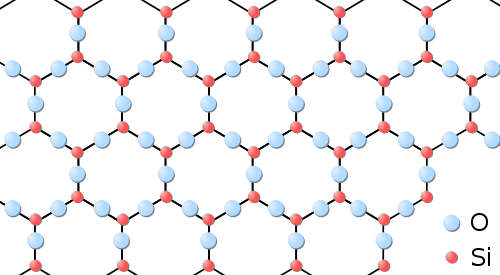
\includegraphics[height=4cm]{Cap_1/500px-SiO2_Quartz.png}}
    \subfloat[Sólido amorfo]{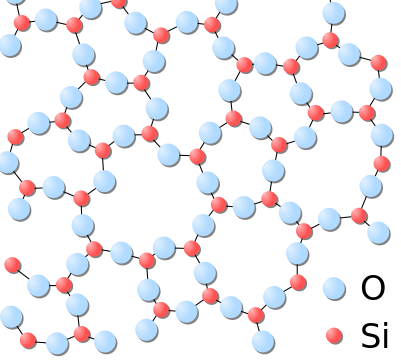
\includegraphics[height=6cm]{Cap_1/500px-Silica.png}}
  \end{tabular}
  \caption[Sólidos cristalinos y amorfos]{Ejemplo de sólido cristalino (Cuarzo) y sólido amorfo (Vidrio). Ambos casos a partir del Sílice (SiO$_{2}$)}
  \label{C1:fg:crystalAmorphous}
\end{figure}

Por otra parte, en cuanto a la composición química, la clasificación está basada en los elementos químicos que los componen. La tabla periódica de los elementos clasifica a los elementos químicos en elementos metálicos, no metálicos y elementos de transición. Un metal está compuesto de uno o más elementos metálicos (y eventualmente elementos no metálicos en muy baja concentración). Los cerámicos, por otro lado, están compuestos de una mezcla de elementos metálicos y no metálicos. 

Estos sólidos, debido a sus diferencias en estructura y composición química, exhiben propiedades mecánicas, térmicas, ópticas, etc. diferentes. Tanto metales como cerámicos suelen contar con una gran rigidez y resistencia. Los cerámicos suelen ser más duros, pero a la vez son más frágiles que los metales y son muy susceptibles a la fractura. En la tabla \ref{C1:tbl:propiedades} se definen algunas de las propiedades mecánicas que normalmente se estudian en ciencia de los materiales.

\begin{table}[htp]
\caption[Nombre y definición de propiedades mecánicas.]{Nombre y definición de propiedades mecánicas normalmente estudiadas en la ciencia de los materiales
\cite{askeland98}.}
\begin{center}
\begin{tabular}{c C{10cm}}
\hline
\textbf{Propiedades Mecánicas} & \textbf{Definición} \\ \hline
 \hline

Elasticidad &
Capacidad de un material a deformarse ante la acción de una carga, recuperando la forma inicial al retirarse la misma. \\ \hline
 
Plasticidad &
Capacidad de un material a deformarse ante la acción de una carga, permaneciendo la deformación al retirarse la misma. \\ \hline 
 
Resistencia & 
Es la medida de la oposición al cambio de forma, a la destrucción del material. \\ \hline

Dureza & 
Resistencia de la superficie de un material a la penetración por un objeto duro.\\ \hline

Ductilidad & 
Capacidad del material a deformarse de manera permanente (deformación plástica) sin romperse. Un material \textbf{dúctil} es lo opuesto a un material \textbf{frágil}. \\ \hline

Tenacidad & 
Capacidad de un material para resistir cargas de impacto. \\ \hline

Resiliencia &
Capacidad de un material de absorver energía antes de fracturarse. \\ \hline

Maleabilidad & 
Capacidad de un material de deformarse sin romperse obteniendo láminas. \\ \hline

Maquinabilidad &
Propiedad de los materiales que permite comparar la facilidad con que pueden ser mecanizados por arranque de virutas. \\ \hline

Esfuerzo de fluencia & 
Esfuerzo aplicado a un material cuando comienza a evidenciarse una deformación plástica permanente.\\ \hline

Rigidez & 
Medida a través del \textit{Módulo de Young}. Pendiente de la curva tensión-deformación en la región elástica. \\ \hline

Moldeabilidad &
Propiedad de un material de adquirir una forma por efecto de una carga, y de conservarla al retirarse la misma. \\ \hline

\end{tabular}
\end{center}
\label{C1:tbl:propiedades}
\end{table}

De lo dicho anteriormente, se observa que tanto los metales como los cerámicos tienen ventajas y deficiencias uno con respecto al otro. Sería lógico entonces intentar combinar ambos tipos de sólido en un único material. Una de las formas de hacerlo es mediante los materiales compuestos. Los materiales compuestos representan una unión macroscópica (e incluso microscópica) de uno o más sólidos clásicos como vemos en la Figura \ref{C1:fg:composite}. Sin embargo, cada una de las partes que componen al material compuesto son un sólido clásico. Para lograr una combinación más fuerte es necesario reducir aún más la escala de trabajo, llegando a la escala nanométrica. Un nanómetro es equivalente a $10^{-9} m$. A modo comparativo, el tamaño promedio de un átomo suele tomarse como de 200 pm, lo cual implicaria que un nanómetro contendría 5 átomos.

\begin{figure}[h!]
 \centering
 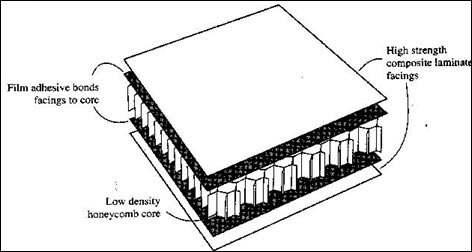
\includegraphics[width=8cm]{Cap_1/compositeCAMBIAR.jpg}
 \caption[Material compuesto]{Esquema general de un material compuesto}
 \label{C1:fg:composite}
\end{figure}

El material denominado vidrio metálico (MG) logra el objetivo de combinar ambos tipos de sólido a escala nanométrica. Se le ha denominado \textit{vidrio} (un material cerámico) debido a su estructura amorfa y \textit{metálico} por tratarse de una aleación de elementos metálicos. Está basado en metales como cobre, níquel, hierro, oro, paladio, titanio, circonio, berilio y lantano; usualmente también se lo combina con bajas proporciones de no metales como boro, silicio, fósforo \cite{andrievski13}.

Cuando un metal se enfría lentamente, se nuclean pequeños cristales que luego crecen a medida que transcurre el tiempo y que la temperatura baja. Este fenómeno se debe a que el material bajo esas condiciones es más estable bajo una estructura ordenada y periódica, es decir, minimiza su energía libre en un estado de sólido cristalino. Sin embargo, existe otro factor que influencia la solidificación: la dinámica o velocidad de enfriamiento. Al enfriar el líquido a velocidades elevadas, la solidificación es lo suficientemente rápida para mantener la estructura desordenada del líquido, es decir, obtenemos un metal amorfo (o vidrio metálico). El hecho de poder obtener una estructura diferente a la cristalina, implica que existe un equilibrio metaestable para una composición dada a cierta temperatura. Esto sucede cuando la energía libre es un mínimo, pero no un mínimo absoluto.

Teóricamente, todo líquido podría convertirse en vidrio a velocidades de enfriamiento suficientemente altas y temperaturas suficientemente bajas evitando el proceso de cristalización \cite{turnbull61}. A lo largo de los años se han ido perfeccionando varias técnicas que actúan sobre la composición, volumen y velocidad de enfriamiento a la que se somete el material, las cuales han permitido la síntesis de vidrios metálicos.

%----------------------------------------------------------------------------------------
%	SECTION 2
%----------------------------------------------------------------------------------------

\section{Producción de aleaciones metálicas amorfas}
\label{S1_2}

Los métodos tradicionales para la preparación de los vidrios metálicos son la solidificación del material fundido sobre una superficie en movimiento, la deposición en substratos fríos y la electrodeposición. Pol Duwez propuso un método para obtener una lámina de metal amorfo a partir de un líquido que pasa a través de dos grandes ruedas de cobre a baja temperatura \cite{duwez60}. Al ser pequeña la relación entre la superficie de contacto del líquido y el volumen, éste se enfría de manera casi instantánea. En un proceso similar (Torneado en estado de fusión o Melt Spinning en inglés), sólo se utiliza un sólo disco giratorio sobre el que se hace impactar un chorro líquido a alta presión sobre la cara exterior de la rueda, logrando velocidades de enfriamiento de hasta $10^{7}$ K/s.

\begin{figure}[h!]
  \centering
  \begin{tabular}{c}
    \subfloat[Maquinaria]{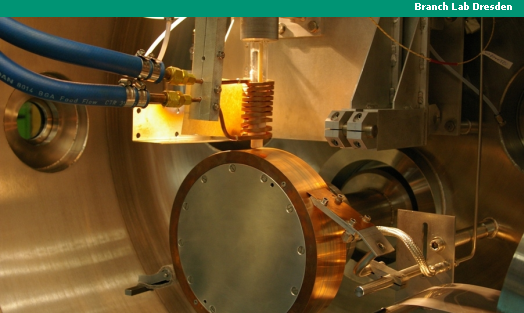
\includegraphics[height=4cm]{Cap_1/melt_spinning_A.png}}
    \vspace{1cm}
    \subfloat[Proceso]{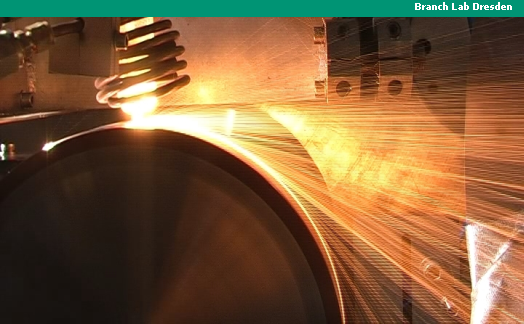
\includegraphics[height=4cm]{Cap_1/melt_spinning_B.png}}
  \end{tabular}
  \caption[Torneado en estado de fusión]{Imágenes del proceso de \textit{Melt Spinnning}. Tomado de Fraunhofer Institute for Manufacturing Technology and Advanced Materials IFAM - http://www.ifam.fraunhofer.de}
  \label{C1:fg:meltSpinning}
\end{figure}

Otra opción es atomizar un líquido y enfriar las pequeñas gotas mediante un gas. Se puede obtener así polvo de vidrio metálico (el cual es necesario sinterizar sin perder las propiedades inducidas por el enfriamiento), o hacer impactar estas gotas contra un molde para crear un sólido de forma directa. Existen métodos comerciales que logran una porosidad tan baja que el material así formado puede luego ser forjado. En la figura \ref{C1:fg:metal_powder} podemos ver un esquema del proceso de atomizado. La sigla \textbf{\textit{VIGA}} significa \textit{\textbf{V}acuum \textbf{I}nduction melting combined with \textbf{G}as \textbf{A}tomization} (fundido por inducción al vacío combinado con atomización por gas) y la sigla \textbf{\textit{EIGA}} significa \textit{\textbf{E}lectrode \textbf{I}nduction melting combined with \textbf{G}as \textbf{A}tomization} (fundido por inducción de electrodo).

\begin{figure}[h!]
 \centering
 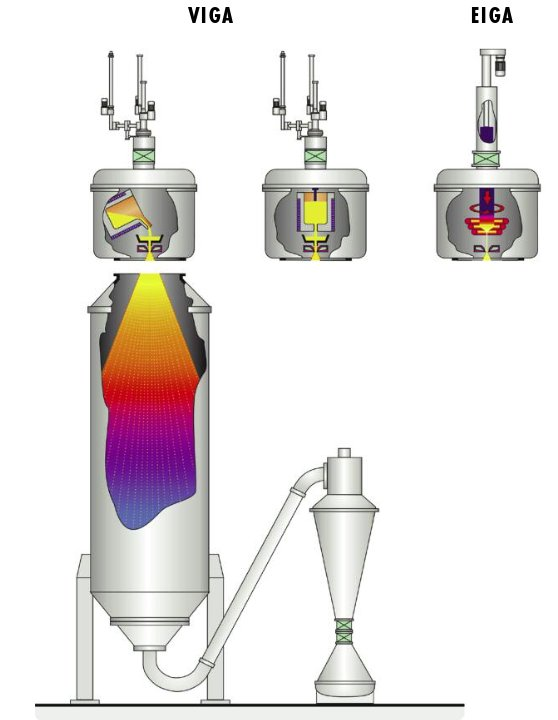
\includegraphics[width=10cm]{Cap_1/metal_powder.jpeg}
 \caption[Atomizado de metal]{Esquema del atomizado de partículas líquidas de una aleación. Tomado de ALD Vacuum Technologies www.ald-vt.de}
 \label{C1:fg:metal_powder}
\end{figure}

Si bien el principio es el mismo, la calidad de la aleación resultante de estos procesos depende fuertemente de la composición del material utilizado, ya que esta afecta en gran medida la capacidad de formación de vidrio del material. Teniendo en cuenta que la extracción rápida de calor de un material es una operación difícil, es de interés encontrar composiciones que permitan producir vidrios a menores velocidades de enfriamiento.

\section{Producción científica}
\label{S1_3}

Podemos decir que a grandes rasgos en la producción científica en torno a los vidrios metálicos se distinguen tres enfoques de trabajo: el modelado de las diferentes propiedades a nivel físico-matemático, la descripción de comportamientos bajo diferentes condiciones de ensayo, y la mejora de las propiedades mecánicas. A continuación de resume la producción científica de los últimos años que sirven de base para este trabajo. Hay que tener presente que algunos de los estudios se realizan en simulación, otros experimentalmente y otros con ambos enfoques a modo de validación. Se puede consultar en las referencias el método particular de cada uno de ellos.

\subsection{Modelado de vidrios metálicos}
\label{S1_3_1}

+Voronoi
+Limiting Strength
+Failure criterion

\subsection{Descripción de comportamiento}
\label{S1_3_2}

\cite{xiao12} observa la mecánica de deformación de MGs en nano-alambres bajo compresión, y cómo la velocidad de enfriamiento afecta la formación de bandas de corte. La tolerancia al daño de los MGs es analizada en \cite{Demetriou11}, en donde se indica que la relación dureza-resistencia de los mismos es comparable a la de los materiales más resistentes conocidos.

Un trabajo que estudia la dependencia de la resistencia y la ductilidad con el tamaño de muestra es \cite{Dongchan10}. En el mismo se realizan ensayos de tracción en nano-alambres de aleaciones basadas en Circonio de diferente diámetro junto con ciclos de carga y descarga.

En un esfuerzo por comprender la dinámica de los átomos de mayor energía de deformación (\textit{atomic strain energy}) \cite{tang15} compara la evolución de los desplazamientos cuadráticos medios entre estos y el de todos. El hecho de que su dinámica sea distinta se ve correlacionada con la respuesta esfuerzo-deformación de los mismos, lo que podría sugerir una relación con la nucleación de STZs y la posterior propagación en SBs.

Esta relación también es estudiada desde otro enfoque en ensayos de nano-indentación. \cite{gu15} estudia la deformación plástica durante el ensayo, observando la propagación de bandas de corte EMBRIONARIAS??? (ESBs) sin la formación de bandas de corte maduras (MSBs) que propaguen a través del material en su totalidad. El fenómeno es atribuido a los tamaños de muestra utilizados, ya que según \cite{shimizu06} existe una escala de longitud intrínseca de unos 100 nm por debajo de la cual la concentración de esfuerzo de corte en la escala de la muestra no ocurre a menos que se utilicen velocidades de deformación muy elevadas (> 10$^{8}$/s), como encontramos en simulaciones de MD comúnmente.

\cite{ma15} estudia la transición amorfo-cristal al someter una muestra de aluminio-hierro (Al$_{50}$Fe$_{50}$) a esfuerzos fluctuantes de tracción. Lo que se observa es que si bien el ensayo se realiza a temperaturas bajas (50 K) partes del material cristalizan luego de cierto número de ciclos. Es interesante este efecto ya que podría darse por sentado que solo a altas temperaturas podríamos encontrarnos con estos efectos (cuando la cristalización ocurre a causa de la difusión activada termicamente) y por consiguiente encontrarnos ante situaciones de falla inesperada.

\subsection{Mejora de propiedades mecánicas}
\label{S1_3_3}

Para controlar y por consiguiente mejorar la dinámica de la plasticidad, se ha modificado tanto la composición como la estructura a escala nano y micro de los vidrios metálicos de diferentes maneras. Cada investigación presenta un enfoque diferente de los mecanismos de deformación según el objetivo del estudio. A veces la generación de SBs se considera deseable (siempre y cuando sean controladas) como es el caso de \cite{chen14} quienes se benefician de las deformaciones plásticas y las micro-fracturas para la disipación de energía y así pensar en su aplicación a dispositivos de absorción de energía.

Por otro lado, muchos trabajos se centran en impedir la propagación de SBs para evitar que el material falle de manera frágil y no controlada. Particularmente, la inclusión de nanopartículas cristalinas provee obstáculos a la propagación y crecimiento de SBs. Ésto se traduce en una deformación más reducida y homogénea en régimen plástico. \cite{albe13} estudia a través de MD los efectos de agregar numerosos nanoprecipitados de cobre cristalino en una matriz amorfa. En este caso las simulaciones se realizan a bajas temperaturas (50 K) y relativamente bajas velocidades de deformación (10$^{7}$ /s).

\cite{brink15} estudian con más detalle los mecanismos de propagación de SBs en un medio con nanopartículas embebidas. Señalan que el tamaño de la inclusión, el esfuerzo necesario para crear dislocaciones en la misma, y la distancia entre precipitados juegan roles conjuntos cuando una SB se propaga. Notan cuatro mecanismos: la partícula se disuelve a estado amorfo por el esfuerzo cortante, la SB rodea a la partícula y sigue su camino, la NP bloquea el paso de la SB y se nuclea en una dirección diferente, la SB corta la nanopartícula produciendo dislocaciones internas. En este trabajo también se analizan casos experimentales a través de Microscopia Electrónica de Transmisión (TEM).

\cite{kuo14} analiza cómo el agregado de precipitados modifica la plasticidad inducida por deformación. Un estudio sobre la formación de esos precipitados mediante recocido se encuentra en \cite{wei14}. En este último, primero se obtiene una matriz amorfa de MG y luego se la recoce alrededor de $T_{g}$ para lograr cristalizar estructuras $B2$ en una proporción cercana a la deseada.

\cite{Zheng12} estudia el incremento de ductilidad en aleaciones cuando se reemplazan átomos por otros diferentes, modificando las propiedades de los enlaces atómicos.

%----------------------------------------------------------------------------------------
%	SECTION 4
%----------------------------------------------------------------------------------------

\section{Propiedades y aplicaciones de los vidrios metálicos}
\label{S1_4}

Como ya se ha dicho, los vidrios metálicos poseen características y propiedades excepcionales que los hacen candidatos para ser usados en artefactos tecnológicos modernos o de alta complejidad.

La tabla~\ref{C1:tbl:props} es una adaptación de un estudio realizado por \cite{ashby06}, en el cual se analizan las propiedades de los vidrios metálicos para su posible aplicación como materiales estructurales.

\begin{table}[htp]
\caption[Propiedades de los vidrios metálicos.]{Propiedades de los vidrios metálicos (adaptada de la tabla en \cite{ashby06}).}
\begin{center}
\begin{tabular}{c C{5cm} C{5cm}}
\hline
\textbf{Atributos} & \textbf{Ventajas} & \textbf{Desventajas} \\ \hline
 \hline

Generales &
Ausencia de efectos adversos debidos a fronteras de granos. &
Alto costo y grandes limitaciones de fabricación \\ \hline
 
Mecánicos &
Alta dureza. Resistencia al desgaste y la abrasión. Gran resistencia mecánica y menor rigidez que las aleaciones cristalinas. Esto le provee una muy alta resiliencia. & 
Gran pérdida de ductilidad ante la aparición de bandas de corte (véase sección~\ref{S1_5}). El recocido (annealing en inglés) lo vuelve frágil. \\ \hline 
 
Térmicos & 
Su baja temperatura de transición vítrea (Tg) permite el tratamiento como líquido superenfriado. & 
Presenta inestabilidad a temperaturas altas (superiores a Tg). \\ \hline

Eléctricos y magnéticos & 
Alta permeabilidad magnética. La resistividad es casi independiente de la temperatura.& 
En campos oscilantes se pierde energía, al ser un material magnetoestrictivo (como aquellos utilizados en transductores).\\ \hline

Químicos & 
Resistencia a la corrosión debido a la falta de bordes de grano.& \\ \hline

Ambientales & 
Algunos MG son biocompatibles & No son fáciles de reciclar. \\ \hline

\end{tabular}
\end{center}
\label{C1:tbl:props}
\end{table}

Es evidente del análisis de la tabla que los vidrios metálicos, en el estado actual de la técnica, sólo son viables en aplicaciones de alto valor agregado, dado su alto costo de fabricación. Por otro lado, hasta que no se mejoraron las técnicas de fabricación no fue posible obtener vidrios metálicos de volúmenes considerables. Por ello las aplicaciones comerciales ``tradicionales'' de estos materiales fueron como revestimiento (debido a su resistencia a la corrosión, el desgaste y las ralladuras) y en transformadores y dando blindaje magnético (debido a las excelentes propiedades magnéticas de los vidrios metálicos basados en Hierro).

Con el surgimiento de nuevas técnicas de fabricación, el interés en estos materiales ha resurgido y las aplicaciones han aumentado en cantidad. Son ampliamente usados en equipamiento deportivo de primera calidad, debido a su relación resistencia-peso y a su gran resiliencia. Estas características permiten que se gaste muy poca energía en la deformación del material y que más energía se transmita.

La biocompatibilidad de algunos vidrios metálicos los hace candidatos para ser utilizados en aplicaciones biomédicas. Otros usos posibles son: sistemas microelectromecánicos (MEMS), electrónica de consumo, aplicaciones aeroespaciales, etc.

\begin{figure}
 \centering
 \begin{tabular}{c}
  \subfloat[Omega Seamaster Edición Limitada]{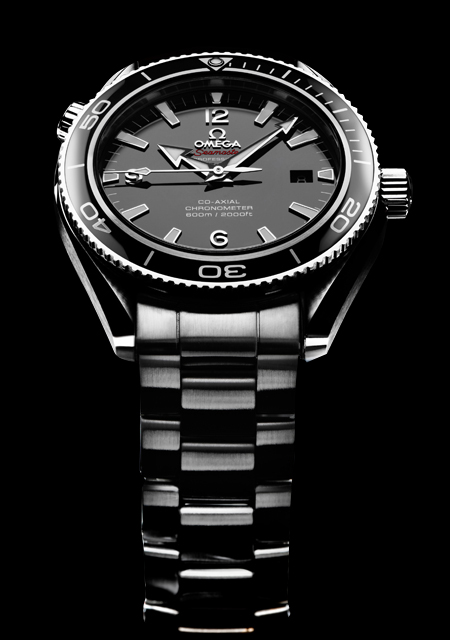
\includegraphics[width=4cm]{Cap_1/seamaster.jpg}}
  \vspace{1cm}
  \subfloat[Otra imagen de aplicación]{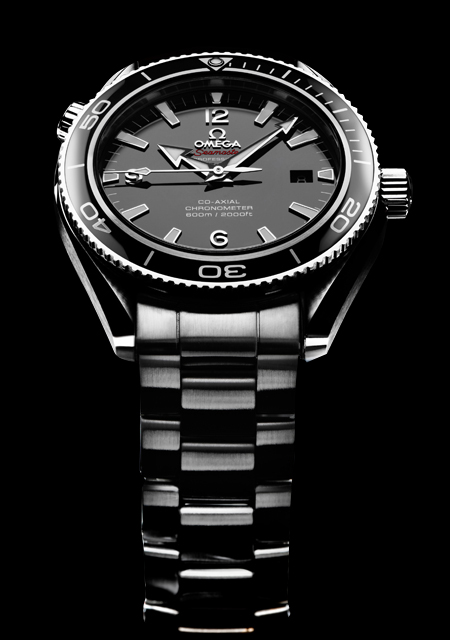
\includegraphics[width=4cm]{Cap_1/seamaster.jpg}} \\
  \subfloat[Otra más ]{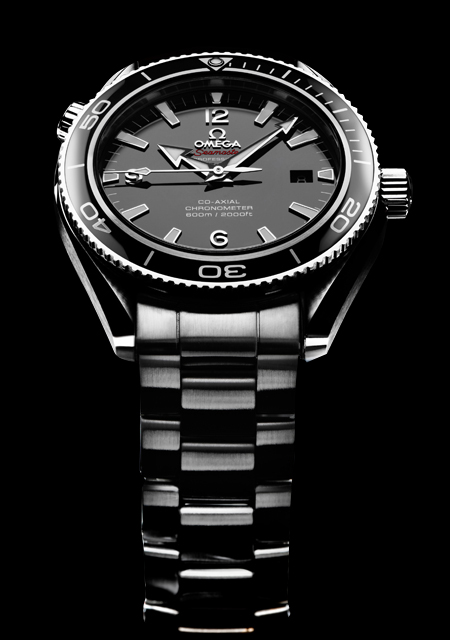
\includegraphics[width=4cm]{Cap_1/seamaster.jpg}}
  \vspace{1cm}
  \subfloat[Y Otra]{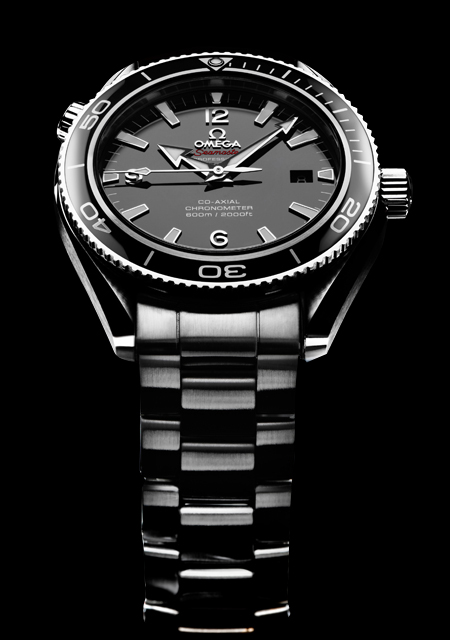
\includegraphics[width=4cm]{Cap_1/seamaster.jpg}} \\
 \end{tabular}
  \caption{Algunos ejemplos de usos actuales de vidrios metálicos}
  \label{C1:fg:usecases}
\end{figure}


%----------------------------------------------------------------------------------------
%	SECTION 5
%----------------------------------------------------------------------------------------

\section{Muestra de vidrio metálico: Cobre-Circonio}
\label{S1_5}

IMAGEN muestra ???

Así como en los metales se habla de \textit{probetas} para los ensayos mecánicos, en las simulaciones de vidrios metálicos se habla de \textit{muestras}. Esto se debe al tamaño \textit{nano} del material utilizado para la simulación (el término muestra suele utilizarse para denominar una pequeña parte de una cantidad mayor de material).

La muestra que se utilizará y servirá de base para otras muestras es una muestra de un vidrio binario, más específicamente \CuZr (Cobre-Circonio), que se manipulará para simular un BMG (Bulk Metallic Glass por sus siglas en inglés). Aquí es necesario explicar los conceptos de BMGs y vidrios binarios de base Cobre.

Los BMGs son vidrios metálicos que tienen una sección transversal de por lo menos algunos milímetros de grosor \cite{suryana11}. Es importante que en ninguna parte del material se presenten fases cristalinas, y es por esto que se ha dedicado mucho estudio a la generación de BMGs. Por el hecho de tener un volumen grande, se deben desarrollar nuevas técnicas que permitan una velocidad de enfriamiento lo suficientemente grande como para poder mantener a todo el volumen de material en estado amorfo.

Una técnica comúnmente usada para lograr que las velocidades de enfriamiento no sean tan extremas es agregar más elementos al vidrio. Es por ello que la mayoría de los BMGs que han sido experimentalmente creados son aleaciones de muchos elementos, como por ejemplo el vidrio Pd$_{40}$Cu$_{30}$Ni$_{10}$P$_{20}$. Sin embargo, algunos sistemas binarios también pueden utilizarse para formar BMGs. Los BMGs basados en metales de transición tardíos (ejemplo Fe, Co, Ni, Cu) presentan ventajas sobre los basados en metales de transición tempranos, como por ejemplo una mayor resistencia y módulo elástico \cite{Xu04}. Por otro lado, los sistemas binarios son útiles para mejorar la eficiencia de formación de BMGs, ya que algunos sistemas multicomponentes podrían reducirse a sistemas binarios para su estudio \cite{Duan05}.

La muestra Cu$_{46}$Zr$_{54}$ usada es prismática, con un total de alrededor de 160000 átomos, creada con una velocidad de enfriamiento de $10^{12}$ K/s, y ya ha sido descrita por \cite{arman10}. En su trabajo, se estudiaron los efectos de ondas de choque en BMGs. La temperatura experimental de transición vitrea (Tg) de este vidrio metálico es 696 K, y su módulo de cizalla experimental (G) es 30 GPa \cite{johnson05}. 

%----------------------------------------------------------------------------------------
%	SECTION 5
%----------------------------------------------------------------------------------------

\section{Mecánica de la deformación de vidrios metálicos}
\label{S1_6}

IMAGEN STZ y SB ???

Una de las mayores limitaciones para el uso de los vidrios metálicos en aplicaciones estructurales está relacionado con su mecánica de deformación. Debido a su estructura amorfa, los vidrios metálicos, a diferencia de las aleaciones cristalinas, no se endurecen con la deformación, sino que les ocurre exactamente lo contrario (\textit{strain softening} en inglés). Este debilitamiento resulta en la concentración de deformación en bandas muy estrechas, llamadas \textbf{bandas de corte} (SB, por sus siglas en inglés). El crecimiento de estas bandas puede causar la fractura frágil del material \cite{schuh07}.

Varias teorías se han desarrollado en el intento de explicar este fenómeno. Tal vez la más aceptada actualmente es la teoría de zonas de transformación de tensión cortante (STZ por sus siglas en inglés: \textit{shear transformation zones}). Las STZ son pequeñas regiones de pocos átomos cuyo posicionamiento y configuración los hace susceptibles a deformaciones plásticas en respuesta a esfuerzos de corte.

Los conceptos fundamentales de la teoría de STZs fueron desarrollados por Argon \cite{argon79}. Luego Falk y Langer \cite{Falk98, Langer07} desarrollaron una teoría dinámica de STZs. En este modelo, ciertas zonas de pocos átomos pueden deformarse plásticamente y quedarse trabadas en este estado deformado, sin poder seguir deformándose en la misma dirección. La formación de STZs puede llegar a ocurrir a iguales velocidades que el bloqueo de las mismas, y bajo esta condición ocurre flujo plástico.

La acumulación de STZs en ciertas direcciones de corte principales produce las bandas de corte (SB). Buena parte del trabajo presentado en la presente tesis se dedica al descubrimiento y la interpretación de las SB, y a la búsqueda de posibles soluciones para evitar la falla frágil.


%----------------------------------------------------------------------------------------
%	SECTION 6
%----------------------------------------------------------------------------------------

\section{Alcances}
\label{S1_7}

En este trabajo nos avocaremos al estudio del régimen elasto-plástico de vidrios metálicos sometidos a esfuerzos de tracción y compresión, el análisis de parámetros constitutivos y modificaciones estructurales que impácten en su comportamiento mecánico.

Nos centraremos en una muestra de Cobre-Circonio (Cu$_{46}$Zr$_{54}$) para la cual tenemos un potencial interatómico descrito correctamente y utilizado ampliamente en la literatura. Los ensayos realizados presentan un sentido y velocidad de deformación constante, es decir, no se relizan ensayos de carga cíclicos. En el caso general, se aplican condiciones de borde periódicas a la muestra en tres dimensiones y sólo se realiza un ensayo con condiciones de borde libres para una comparación puntual.

El estudio de esta muestra amorfa es puramente numérico, no realizamos ensayos con aleaciones en laboratorio. Sin embargo, esto no quita validez física a las simulaciones de MD siempre que se definan correctamente los parámetros de trabajo.


%----------------------------------------------------------------------------------------
%	SECTION 7
%----------------------------------------------------------------------------------------

\section{Objetivos}
\label{S1_8}

\begin{itemize}
 \item Comprender la metodología de las simulaciones de MD
 \begin{itemize}
  \item Estudiar los principios de dichas simulaciones.
  \item Desarrollar las técnicas de pre/post procesamiento de la información obtenida.
 \end{itemize}
 \item Describir el comportamiento en régimen elasto-plástico de un metal amorfo a diferentes temperaturas.
 \begin{itemize}
  \item Analizar los esfuerzos y deformaciones en régimen plástico.
  \item Obtener curvas de comportamiento frente a la temperatura de diferentes parámetros.
 \end{itemize}
 \item Describir los efectos de cambios en la composición de la muestra sobre las propiedades mecánicas.
 \begin{itemize}
  \item Generar nuevas muestras modificadas: muestras de porosidad variable y muestras con inclusiones cristalinas.
  \item Analizar el comportamiento general de la muestra modificada bajo esfuerzos, a diferentes temperaturas.
  \item Analizar el comportamiento particular de las inclusiones/poros sometidos a esfuerzos, a diferentes temperaturas.
 \end{itemize}
 \item Divulgar los resultados obtenidos en publicaciones científicas.
\end{itemize}

%----------------------------------------------------------------------------------------
%	SECTION 9
%----------------------------------------------------------------------------------------

\section{Metodología}
\label{S1_9}

Se hace uso de simulaciones de MD mediante el paquete LAMMPS \cite{plimpton95}, que es de código abierto y gratuito. Se prepara un script de entrada que describe la simulación (ver Apéndice \ref{AA}) y una vez comprobado que su ejecución es correcta, se generan copias con parámetros diferentes, como por ejemplo la temperatura de simulación.

Se generan dos tipos de archivos de salida. Por un lado tenemos una salida de variables termódinámicas, es decir, cómputos promedios de la muestra completa como la temperatura, la energía potencial, las dimensiones y las componentes del tensor de esfuerzos. Se los denomina generalmente archivos \textit{out} o \textit{log}. Por otro lado nos encotnramos con archivos que contienen propiedades similares pero para cáda átomo. Estos últimos son de un tamaño considerablemente mayor y representan el comportamiento atómico en detalle, ya que contienen información de las posiciones, velocidades, tensor de esfuerzo y energías. Se los denomina arhivos \textit{dump}.

Sobre los archivos \textit{out} se realiza un post procesamiento para calcular propiedades derivadas (por ejemplo el esfuerzo de von Mises) antes de pasar a una representación gráfica. Los archivos \textit{dump} son tratados de manera similar, pero se representan mediante un  software dedicado, que en nuestro caso es Ovito \citep{stukowski10} (ver Apéndice \ref{AB}).

%----------------------------------------------------------------------------------------
%	SECTION 10
%----------------------------------------------------------------------------------------

\section{Contenidos}
\label{S1_10}

El presente trabajo se divide en cinco capítulos y tres apéndices. Una presentación teórica se encentra en el Capítulo \ref{C2}. Los Capítulos \ref{C3} a \ref{C5} engloban el trabajo realizado, presentando cada uno de los diferentes casos de análisis. Las conclusiones finales pueden encontrarse en el Capítulo \ref{C6}. Los Apéndices \ref{AA} a \ref{AC} dan una introducción a las herramientas utilizadas en este trabajo.

El Capítulo \ref{C2} presenta los fundamentos teóricos de las simulaciones de MD, gracias a las cuales se pueden realizar nuestros ensayos computacionales. Se muestran algunos algoritmos utilizados internamente por LAMMPS y las ecuaciones que describen las interacciones atómicas de nuestra muestra.

El Capítulo \ref{C3} detalla los resultados obtenidos al simular la muestra de \CuZr bajo diferentes modos de carga y temperaturas. Se muestran curvas de esfuerzo-deformación, tendencias de módulo de Young y esfuerzo máximo contra temperatura, entre otros.

En el Capítulo \ref{C4} se analiza la estabilidad de nanopartículas cristalinas embebidas en la matriz amorfa original. Se realizan cálculos de difusividad del cristal en la matriz y se compara el comportamiento mecánico de la muestra con este agregado frente a las respuestas originales.

En el Capítulo \ref{C5} se estudia la mecánica de deformación y de cierre de los poros en una matriz de porosidad variable, así como la respuesta mecánica de la muestra en su totalidad frente a la matriz amorfa original. 

El Apéndice \ref{AA} contiene los lineamientos generales para la compilación y utilización del software de simulación elegido (LAMMPS). En el Apéndice \ref{AB} se describe el modo de uso del software de visualización Ovito. Finalmente, en el Apéndice \ref{AC} se da una pequeña introducción a técnicas de \textit{scripting} para pre y post procesamiento de datos de salida.